\begin{surferPage}[Chmutov-Oktik]{Eine Chmutov-Oktik}
    Auf den ersten Blick sieht man, dass Chmutovs Oktik $\text{Chm}_{d}, \ d=8,$
    sehr symmetrisch ist.
    Auch in der Gleichung kann man dies recht leicht erkennen:
    \[\text{Chm}_{d}\colon T_d(x) + T_d(y) + T_d(z) + 1 = 0.\]
    wobei $T_d$ das sogenannte Tchebychev Polynom ist (Bild links).
    Die Kurve $T_8(x)+T_8(y)=0$ sieht man rechts:
    \begin{center}
      \begin{tabular}{c@{\quad}c}
        \begin{tabular}{c}
          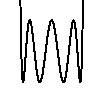
\includegraphics[height=1.75cm]{./../../common/images/Tcheb_008.pdf}
        \end{tabular}    
        &
        \begin{tabular}{c}
          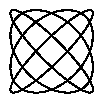
\includegraphics[height=1.75cm]{./../../common/images/Tcheb_2d_008.pdf}
        \end{tabular}    
      \end{tabular}
    \end{center}
    \vspace{-0.3cm}
    Von diesen Bildern zum Aussehen der Fläche ist es nicht mehr allzu weit. 

    Diese Gleichungen hat V.\ Chmutov Anfang der 80er Jahre gefunden. 
    Damals stellten sie für fast alle Grade $d$ den Weltrekord für $\mu(d)$,
    also für die maximale Anzahl von Singularitäten auf einer Fläche vom Grad
    $d$ dar.
    In den 90ern hat er selbst seinen Rekord verbessert und 2005 haben S.\
    Breske, O.\ Labs und D.\ van Straten diese Konstruktion auch für reelle
    Singularitäten durchgeführt.
\end{surferPage}
